\subsection{Bonding Quality Tests}
INTRO HERE + DEFINITIONS AND DIFERENCES (GOSELE ET AL WAFER 
DIRECT BONDING)
\subsubsection{Bonding Energy Test}
\subsubsection{Bonding Strength Test}
One of the most widely used methods to assess bonding strength 
is the \textit{tensile test} (also known as the pull test or 
direct tensile method). In this approach, bonded substrates
are attached to two separate fixtures using a high-strength adhesive. 
These fixtures are then pulled apart in a direction perpendicular 
to the bonding interface, applying tensile stress that tends to 
separate the bonded wafers. A typical experimental setup 
is shown in Figure \ref{fig:tensile_test} \cite{wasmer2007,muller1991}.

\begin{figure}[h]
\centering
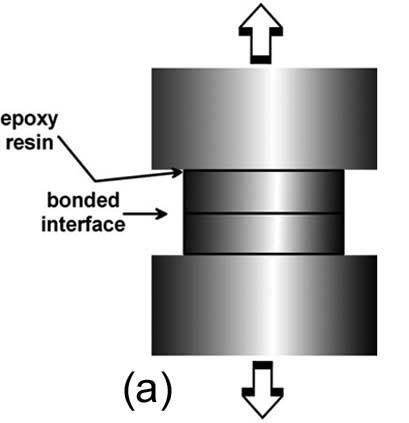
\includegraphics[width=0.5\textwidth]{Images/tensile_test.jpeg}
\caption{Schematic diagram of the tensile test setup for bonding 
strength measurement. The bonded wafer pair is glued to metal fixtures 
and subjected to perpendicular tensile force. Adapted from \cite{gosele2006}.}
\label{fig:tensile_test}
\end{figure}

\paragraph{Fracture Mechanics Analysis}
Assuming that the bonding strength is lower than the adhesive's 
strength, cracks will be produced at the bonding interface when 
a certain strength threshold is exceeded. The fracture behavior 
can be characterized using linear elastic fracture mechanics (LEFM). 
Depending on the crack length, a \textit{stress intensity factor} 
($K_I$) can be estimated using the following expression 
\cite{wasmer2007,gosele2006}:

\begin{equation}
    K_I=\sigma Y\left(\frac{a}{\omega}\right)\sqrt{\pi a}
    \label{eq:stress_intensity}
\end{equation}

\noindent where $a$ is the crack length, $\sigma$ is the 
applied stress, and $\omega$ is the substrate width. 
The dimensionless parameter $Y\left(\frac{a}{\omega}\right)$ 
is a geometric correction factor that accounts for the 
finite geometry of the wafer and the crack position. 
For standard edge cracks (the most common failure mode), 
$Y \approx 1.12$ \cite{anderson2005}. 
For internal cracks located far from the edge, 
$Y \approx 1.0$ \cite{anderson2005}.

\paragraph{Crack Propagation Criterion}
Cracks will propagate along the interface ---and therefore 
cause complete fracture--- if the stress intensity factor 
exceeds the material's fracture toughness limit 
($K_I > K_{IC}$). This critical value often depends on 
several parameters, including the crystallographic 
orientation of the material, temperature, loading rate, 
and environmental conditions \cite{wasmer2007,boniecki2001}.

For brittle materials under mode I loading (tensile opening), 
the fracture toughness can be theoretically estimated 
in terms of the surface energy ($\gamma$) as 
\cite{gosele2006}:

\begin{equation}
    K_{IC}=\sqrt{\frac{2E\gamma}{(1-\nu^{2})}}
    \label{eq:fracture_toughness}
\end{equation}

\noindent where $E$ is the Young's modulus and $\nu$ is 
the Poisson ratio of the material.

From Equations \ref{eq:stress_intensity} and 
\ref{eq:fracture_toughness}, a critical stress 
($\sigma_{C}$) for crack propagation can be derived:

\begin{equation}
\sigma_{C}=\sqrt{\frac{2E\gamma}{Y^2\left(\frac{a}{\omega}\right)\pi a(1-\nu^{2})}}
\label{eq:critical_stress}
\end{equation}

\noindent This critical stress represents the bonding strength 
that can be experimentally measured.

\paragraph{Advantages and Limitations}
The tensile test offers several advantages, including 
experimental simplicity, direct measurement of bonding strength, 
and straightforward interpretation based on well-established 
fracture mechanics principles \cite{muller1991}. However, 
several limitations must be considered:

\begin{itemize}
    \item \textbf{High measurement variance:} Real experiments 
    exhibit significant scatter in bonding strength values, 
    which can be attributed to local variations in surface 
    parameters such as roughness, total thickness variation 
    (TTV), particle contamination, and bonding defects 
    \cite{muller1991,gosele2006}.
    
    \item \textbf{Edge effects:} Stress concentrations at 
    wafer edges can lead to premature failure that does 
    not accurately represent the average bonding quality 
    \cite{wasmer2007}.
    
    \item \textbf{Adhesive influence:} The test results 
    may be affected by the properties of the adhesive 
    used to attach the fixtures, particularly if the 
    adhesive fails before the bond \cite{muller1991}.
    
    \item \textbf{Sample preparation:} Careful alignment 
    is crucial to ensure purely tensile loading; any 
    misalignment introduces bending moments that affect 
    the results.
\end{itemize}

Therefore, while the tensile test provides a useful 
estimate of bonding strength, results should be 
interpreted as indicative values rather than absolute 
measurements. Multiple samples and complementary 
characterization methods (such as the razor blade test) 
are recommended for 
comprehensive bonding quality assessment.
\textbf{INCLUDE OUR OWN EXPERIMENT HERE}




